\documentclass[../Main.tex]{subfiles}
\begin{document}

\section{Result in guests}

\subsection{Main page}

\begin{figure}[H]
    \centering
    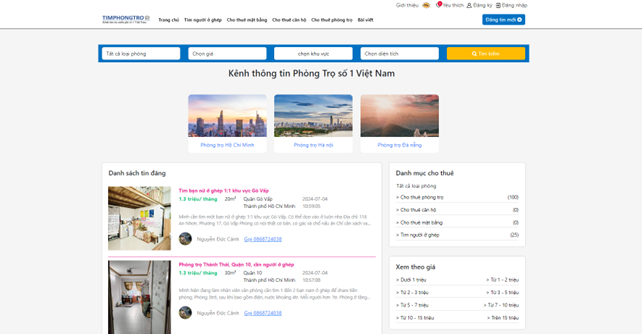
\includegraphics[width=\textwidth]{Figure/Picture21.png}
    \caption{Main page}
\end{figure}

\subsection{Search hostel}

Customers can choose several criteria in the search bar to filter the hostel or click on each category in the right of the system.

\begin{enumerate}
    \item Catagory
          \begin{figure}[H]
              \centering
              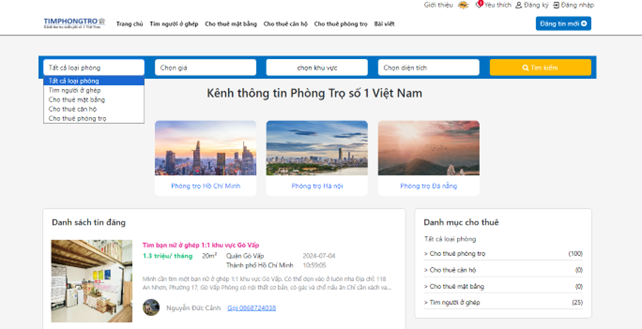
\includegraphics[width=\textwidth]{Figure/Picture22.png}
              \caption{Search by Catagory}
          \end{figure}
    \item Price
          \begin{figure}[H]
              \centering
              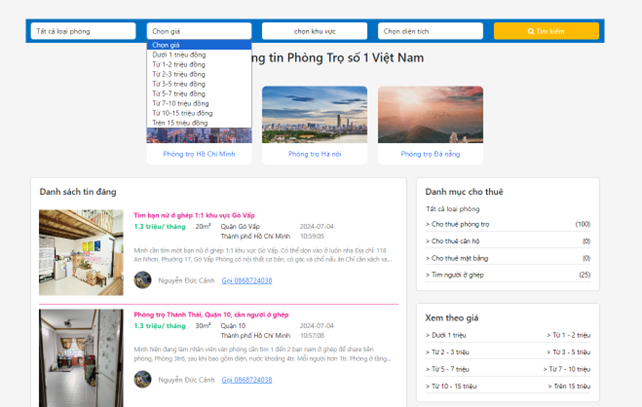
\includegraphics[width=\textwidth]{Figure/Picture23.png}
              \caption{Search by Price}
          \end{figure}
    \item Location.
          In the search bar, customers can choose location to commune level
          \begin{figure}[H]
              \centering
              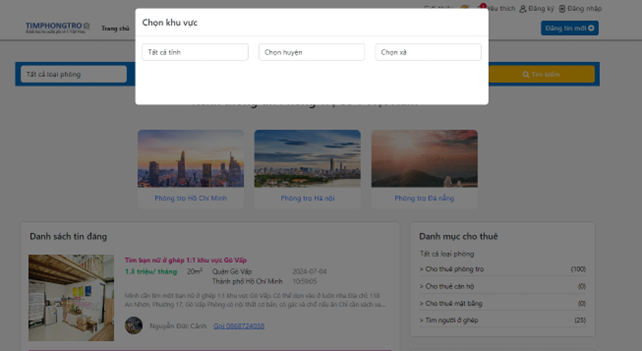
\includegraphics[width=\textwidth]{Figure/Picture24.png}
              \caption{Search by Location}
          \end{figure}
    \item Area
          In the search bar, customers can choose location to commune level
          \begin{figure}[H]
              \centering
              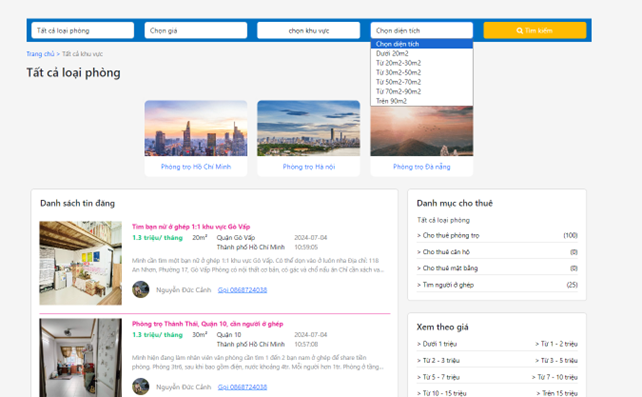
\includegraphics[width=\textwidth]{Figure/Picture25.png}
              \caption{Search by Area}
          \end{figure}
\end{enumerate}

\subsection{See detail hostel}

When users click on any post, the system will direct users to the page illustrating details of this hostel.

\begin{figure}[H]
    \centering
    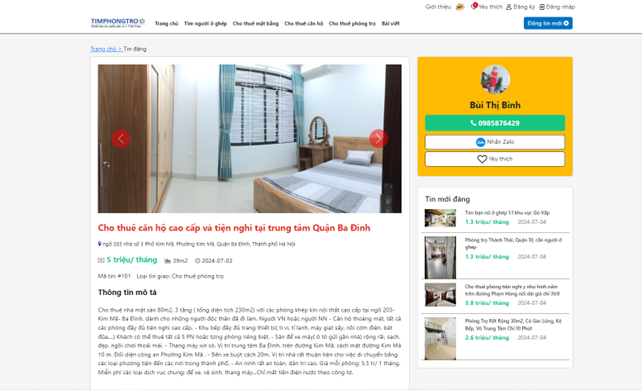
\includegraphics[width=\textwidth]{Figure/Picture26.png}
    \caption{Detail Hostel}
\end{figure}

Here is the information about a hostel.
Beside details hostel, customers can see the information of owner hostel to contact.

\section{Result in users}

When customers want to post room or want find roommates.
They must login/register.

\subsection{Login page}

When customers click on login in the right top conner, the system will direct them to the login page.

\begin{figure}[H]
    \centering
    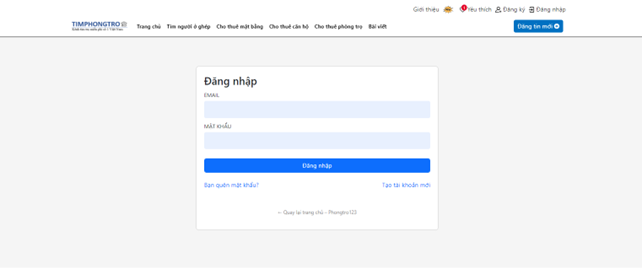
\includegraphics[width=\textwidth]{Figure/Picture27.png}
    \caption{Login Page}
\end{figure}

\subsection{Registration page}

When customers want to login, but they do not have an account, they can click to register in the login page or in main page.

\begin{figure}[H]
    \centering
    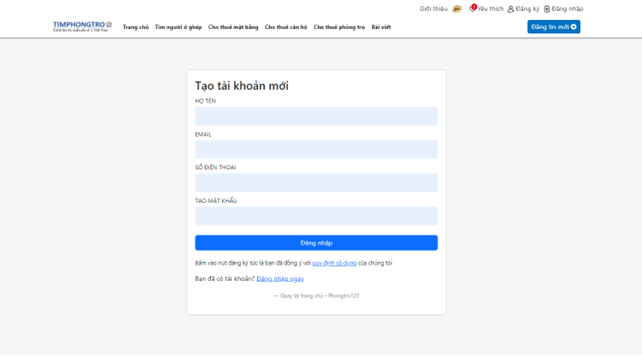
\includegraphics[width=\textwidth]{Figure/Picture28.png}
    \caption{Registration page}
\end{figure}

\subsection{Email Confirmation}

After registering successfully, the system will notice for the user to check email to confirm.

\begin{figure}[H]
    \centering
    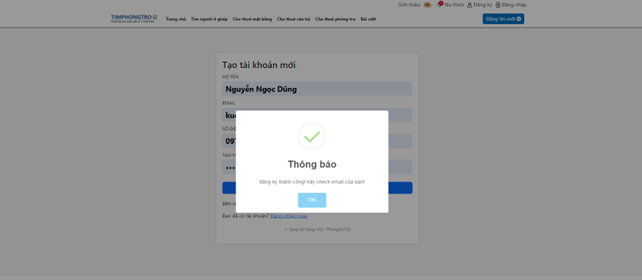
\includegraphics[width=\textwidth]{Figure/Picture29.png}
    \caption{Email Confirmation page}
\end{figure}

Email Confirmation

\begin{figure}[H]
    \centering
    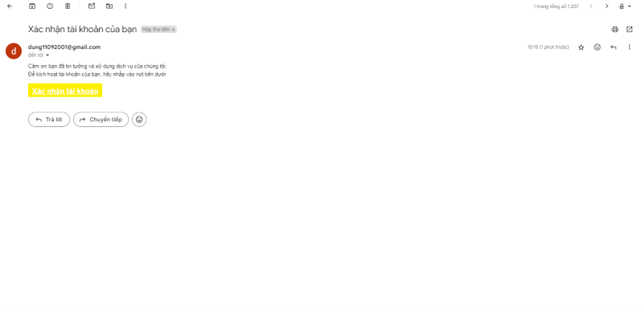
\includegraphics[width=\textwidth]{Figure/Picture30.png}
    \caption{Email Confirmation}
\end{figure}

When user clicks on confirmation account, the system will active user’ account and user can login with this account to this website.

\subsection{Forgot password}

If users forget password, they can click on forget password.

\begin{figure}[H]
    \centering
    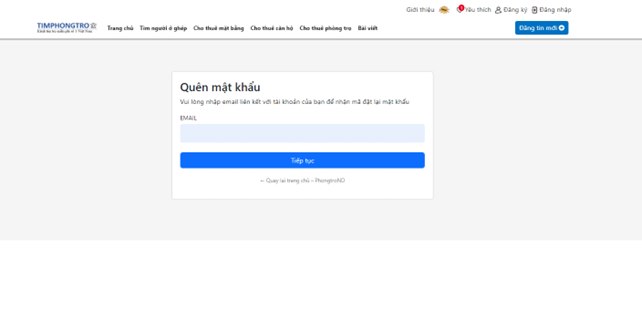
\includegraphics[width=\textwidth]{Figure/Picture31.png}
    \caption{Forgot Password}
\end{figure}

After users enter email address.
They click on Continue to receive new password in their email.

\begin{figure}[H]
    \centering
    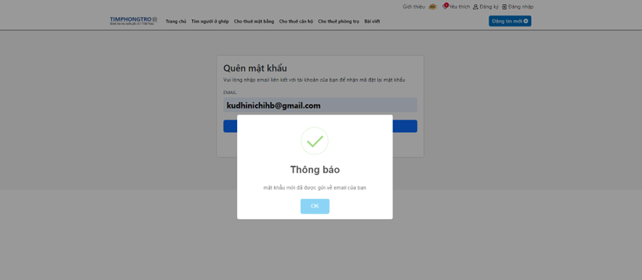
\includegraphics[width=\textwidth]{Figure/Picture32.png}
    \caption{New Password Notification}
\end{figure}

Email template to receive new password

\begin{figure}[H]
    \centering
    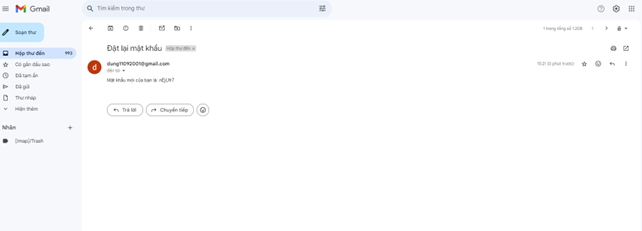
\includegraphics[width=\textwidth]{Figure/Picture33.png}
    \caption{New Password}
\end{figure}

\subsection{Post Hostel Page}

After login, if users want to post their hostel, they click on ``Post new hostel'' in main page.

\begin{figure}[H]
    \centering
    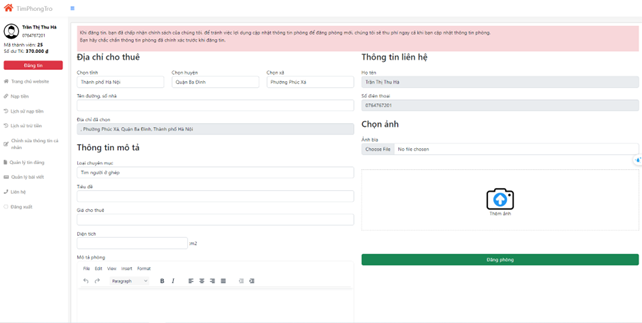
\includegraphics[width=\textwidth]{Figure/Picture34.png}
    \caption{Post hostel page}
\end{figure}

Users must fill all the information like location, category, title \dots to post a hostel.
If the information is valid, the system will notice ``user posts hostel successfully''.

\begin{figure}[H]
    \centering
    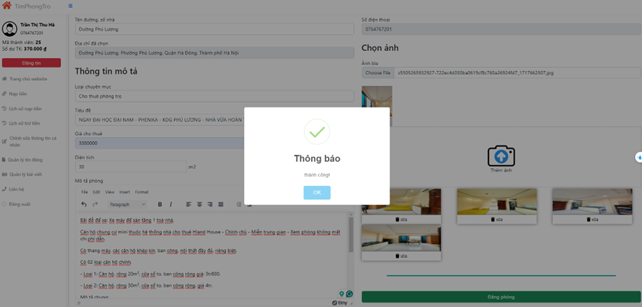
\includegraphics[width=\textwidth]{Figure/Picture35.png}
    \caption{Post hostel page successfully}
\end{figure}

\subsection{Update Hostel Page}

When landlord miss or fill wrong information of this hostel, they click on edit button to fix this wrong information.
The system will direct to post hostel page.

\begin{figure}[H]
    \centering
    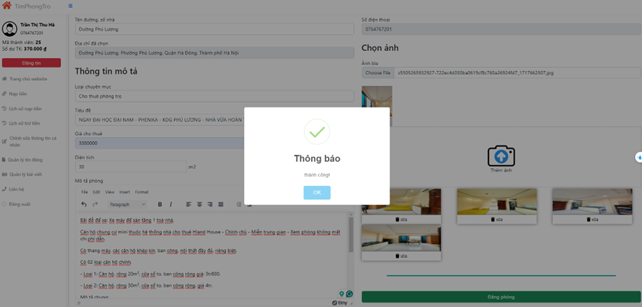
\includegraphics[width=\textwidth]{Figure/Picture35.png}
    \caption{Post hostel page successfully}
\end{figure}

\subsection{Delete Hostel Page}

When users click button delete in particular room, the system will delete it and notice for owner.

\begin{figure}[H]
    \centering
    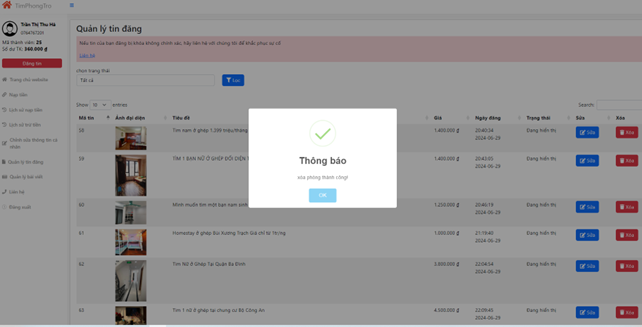
\includegraphics[width=\textwidth]{Figure/Picture38.png}
    \caption{Post hostel page successfully}
\end{figure}

\subsection{User information page }

Users can check their information on the user information page.
They can change name, phone or update avatar, link Facebook.

\begin{figure}[H]
    \centering
    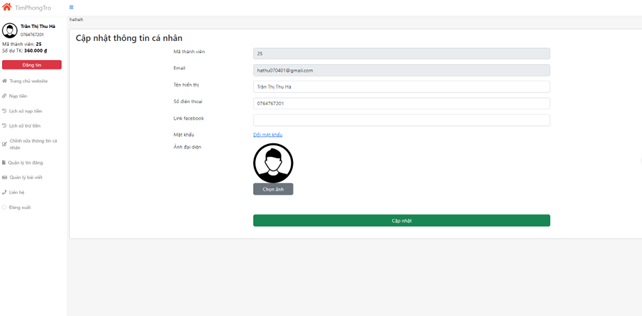
\includegraphics[width=\textwidth]{Figure/Picture39.png}
    \caption{Post hostel page successfully}
\end{figure}

\subsection{Changing password page }

\begin{figure}[H]
    \centering
    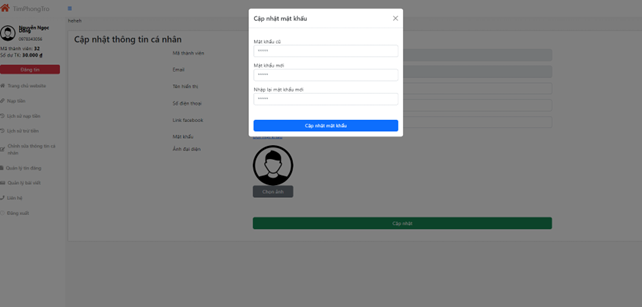
\includegraphics[width=\textwidth]{Figure/Picture40.png}
    \caption{Post hostel page successfully}
\end{figure}

\end{document}
